\section{Introduction}
Car is one of the major vehicles in this modern era of life. Cruising for parking has been shown to be one of the biggest contributors of road congestion and pollution. But day by day the number of cars is increasing in Bangladesh. A statistic shows that total number of private passenger cars in Bangladesh in 2014 was 14699 but within 3 years in 2017 the number rose to 21959. This increased number of vehicles are arising the parking problem. Consequently, this is creating traffic jam, air pollution, wastage of valuable time. Traffic jam is one of our major disadvantages every day.
Although most homes and apartments in Dhaka demand resident parking space, there are still relatively limited rooms for car parking in a wide variety of workplaces, corporations, hospitals, educational institutions and malls. Due to unregulated expansion, there are still very little parking space in a big percentage of the commercial high-rise buildings. Parking cars on surrounding roads and pathways therefore generate unfair traffic jams. In certain areas, merely dropping off and pickup is sufficient to stop traffic movements.
Unplanned and unauthorized parking is the major factor behind this problem. Even if parking arrangements exist, people experience many undesirable occurrences because of inappropriate administration. In our nation, parking systems are less efficient to inform us whether there is space inside while we are outside. Despite obstacles, many accidents occur through human control. Furthermore, the car park is difficult to keep unauthorized individuals free. So car robbing is not a concept that is unknown to us. There are also privilege/VIP parking facilities to be worried about. The management of parking by guards is often hazardous and problematic. Even a simple parking lot requires an active workforce of 2-3 personnel and a manager.
Resolving these issues is a major challenge at a time. It is a more complicated problem to accomplish this manually. Keeping all these in mind, an android based smartphone application is being proposed here that will help to introduce an automatic system for parking. This application will provide the opportunity of reducing wastage of time in parking, more security, lessening the parking expenses etc.
We used android studio Environment (IDE) for developing Android app.
The above-mentioned system will be useful for all to ensure the efficient parking in specific parking slot within a short time.

\section{Framework/Design Overview}
We developed a smart parking system where the parking slot status can be known from android application. Infrared obstacle sensor is used for checking the slot is free or not. Arduino mega2560 is used as a controller. It collects all the data from sensors and after processing those data it displays the slot status. A keyboard is used for inputting password. ESP8266 NodeMCU is used for sending and receiving data to server via internet. When a vehicle comes to parking spot, the user has to register in this system giving his mobile number and vehicle serial. An account is opened simultaneously to server. With this application user can see the slot status and pricing. User can choose a slot and when a slot is requested, a password is generated and shown to user. This password is to be input in smart parking device's keyboard. If the password is matched then parking slot's gate is opened and user can park car here and time counting started. At the time of unpark the application has to be used which was used for parking. When "Unpark" button is pressed the parking duration is calculated and multiplying this duration with slot pricing to calculate bill. From account this bill is deducted. If someone steal the car from parked, a notification to user android application is gone with alarm and vibration. Also an early alarm is given to smart parking system's device.

\section{Difficulties}
In this system many sensors, controller, and keyboard is used. WiFi network is used for internet supply. Thus this parking system works at day and night it needs continuous electricity supply. Again database should be private and secured thus anybody can not access to database. To receive and send data to cloud server uninterrupted internet connection is needed.
The more difficulties are given below:
\begin{itemize}
    \item The application interface should be interactive and user friendly
    \item The whole system should be simple thus complexity is to be minimum and works perfectly
    \item Good quality sensor should be used, otherwise system will work bad.
    \item This system should be at low cost
\end{itemize}

\begin{figure}[H]
\centering
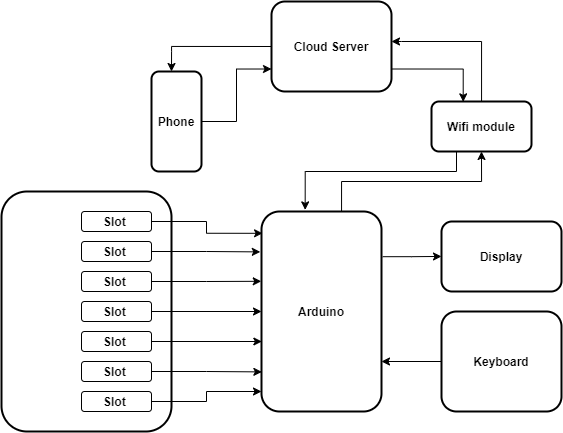
\includegraphics[width=1.0\textwidth]{figures/BlockDig.png}
\caption{Block diagram of the proposed system.}
\label{block}
\end{figure}


\section{Applications}
This system can be used in many cases such as:
\begin{itemize}
    \item Smart car parking system can be used at every parking spot
    \item In urban and rural parking places this system can be used 
    \item In shopping malls, office areas, restaurants this system can be used
\end{itemize}

\section{Motivation}
Nowadays the number of cars is increasing rapidly. The population density is also growing alarmingly. Many drivers do not know the nearest parking space for this reason they waste a lot of time for searching the nearest parking space. Again for difficulties of searching parking space, many people park their car on footpath thus the road gets narrower. So vehicles can not move smoothly which causes accidents and by finding parking spot extra fuel is burnt and produce air pollution. According to statistics every day 3000 gallons of fuel are burnt for searching parking place\cite{}. Moreover, parking a car at a random place makes it easier to steal. In the previous works, RFID was used but RFID is not always possible to carry so we got motivated from those problems to develop a smart car parking system. 

\section{Objectives}
The main objectives of our thesis are given below:
\begin{itemize}
    \item To find parking spot easily 
    \item To reduce human hassle
    \item To make parking process automated and faster
    \item To make different slot price according to slots distance 
\end{itemize}

\section{Contribution of the thesis}
\begin{itemize}
    \item Developing a mobile application that provides different emergency and non-emergency parking slots for various needy users by varying user preferences and slot availability.
    \item Designing a model that can prevent car theft by using the antitheft alarm through SMS, Buzzer, and Alert Notification on a smartphone.
    \item Designing a model that allows parking slot users to pay the bill automatically by using mobile banking.
    \item Designing an automated system that allows services like App installation and registration, Booking Procedure, Entrance Procedure and Parking slot allocation.
\end{itemize}

\section{Thesis Organization}
This paper has five chapters. In chapter 1 describes some introductory description, design framework, application, motivation, history, implementation difficulties and contributions of the proposed system. Chapter 2 gives an overview
of the literature review and hardware component description, implementation
challenges about this proposed system. Chapter 3 discusses the system architecture, methodology, hardware components role, software components role and
android application regarding this system. Chapter 4 describes the experimental
results, impacts and performance evaluation of the system. Chapter 5 presents
the conclusions, limitations and future recommendations regarding this.

\section{Conclusion}
In this chapter a brief discussion on smart parking system using internet of things is written. Also, the problems of present parking situation are discussed. The motivation behind this thesis is also written here. The objectives and our contribution to this thesis are also written. In the following chapters, we will discuss this work in detail.  